\section{Graph Embeddings for Traffic Scene Analysis}
\label{chapter:implementation_of_graph_embeddings_for_traffic_scene_analysis}

This section describes the concepts, implementation and application of graph embeddings to traffic scene graphs. 
The implementation follows a comprehensive approach to learning graph representations through self-supervised 
contrastive learning.

Embeddings are a widely used method to translate raw data like images or text into an embedding space in order to be 
able to perform machine learning tasks on them. One well known example of this is the Word2Vec model, which is used to 
translate words into a 
vector space, where the distance between vectors can be used to measure the similarity between 
words (\cite{mikolov2013efficientestimationwordrepresentations}).

In the context of traffic scene graphs, embeddings are used to translate the graph structure into a vector space, 
where the distance between vectors can be used to measure the similarity between traffic scenes.
This is useful for coverage analysis, as it allows to compare traffic scenes among each other.
For example, two traffic scenes can be considered similar if the distance between their embeddings is small. This enables
to search for a most similar simulation scenario given a real world scenario, to identify areas with near duplicates or 
to easily visualize structures in the embedding space, which in the original space of all possible traffic scenes
would not be possible.

Graph neural networks (GNNs) are a class of neural networks that are designed to process graph-structured data and have 
gained a lot of popularity in the last years, see for example (add references).

In this paper, a network architecture using a Graph Isomorphism Network with Edge features (GINE) as described 
in \cite{hu2020strategiespretraininggraphneural} is used to generate embeddings for traffic scene graphs as implemented in the 
pytorch geometric library (\cite{Fey/Lenssen/2019}). Main reason for using this specific architecture is that is capable of
learning embedding representations not only on the graph structure itself but on both node and edge attributes. Other 
network architectures like GraphSAGE or GAT are not capable of this. (TODO: check if this is true)

\begin{figure}[h]
    \centering
    %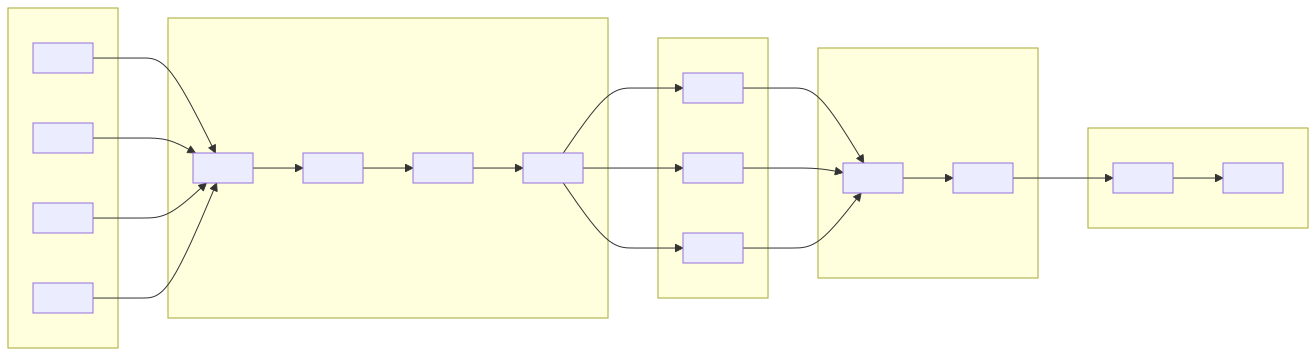
\includegraphics[width=0.8\textwidth]{plots/graph_gine_architecture.pdf}
    \includegraphics[width=0.8\textwidth]{plots/graph_gine_architecture_manually_updated.png}
    \caption{Model architecture for the Graph Isomorphism Network with Edge features (GINE).}
    \label{fig:graph_gine_architecture}
\end{figure}

The exact architecture of the model is shown in Figure \ref{fig:graph_gine_architecture}. The features 
used are the actor type (as a one hot encoding),
the actor speed (float), if the actor is on an intersection (boolean) and if the actor changed its 
lane since the last timestep (boolean) for the nodes.
For the edges, the edge type (as a one hot encoding) and the path length (float) between the two nodes are used.

The model has been trained on the CARLA and Argoverse 2.0 datasets using self-supervised contrastive learning. 


Training employed a self-supervised contrastive objective on mini-batches of 128 graphs. 
For each batch, two correlated views of every graph were created by 
perturbing continuous attributes with zero-mean Gaussian noise ($\sigma=0.1$) applied to node 
longitudinal speed and edge path length. A four-layer GINE encoder 
(hidden width 96) produced graph-level representations via the concatenation of 
mean, max, and sum pooling, followed by an embedding MLP (yielding 256-dimensional embeddings) and a projection head. The contrastive loss was a temperature-scaled cross-entropy over in-batch similarities (cosine similarity of $\ell_2$-normalized projections, temperature $\tau=0.1$), maximizing agreement of the two views of the same graph while contrasting against other graphs in the batch. Optimization used Adam with an exponentially decaying learning rate, initialized at 0.02 and multiplied by 0.75 across successive stages. 
This setup follows established practice in contrastive pretraining for GNNs \cite{hu2020strategiespretraininggraphneural} 
and is implemented using PyTorch Geometric \cite{Fey/Lenssen/2019}.

